\documentclass[11pt,a4paper,titlepage]{article}
\usepackage{subscript,subfigure,amsmath,amssymb,tabularx,amstext,amsfonts,mathrsfs,graphicx}

\begin{document}

\title{GEP Protokoll - Laborversuch 7\\[1ex]
Operationsverst\"arker}
\author{Cao Thi Huyen \and Robert R\"osler \and Nico Grimm}
\date{04. Januar 2016}

\maketitle

% --- Aufgabe 1 ---
\section{Nicht-invertierender Verst\"arker}
In diesem Versuch lernen wir grundlegende Kenntnisse \"uber einen OP-Verst\"arker kennen und \"uben die Anwendung mit einfachen Grundschaltungen. \\[1ex]
Die Kenndaten unseres Operationsverst\"arker:
\begin{itemize}
\item OPV Typ: CA3140
\item Impedanz (unbeschaltet): $Z_{ein}=1,5T\Omega, Z_{out}=60\Omega$
\item Betriebsspannung: ±15V
\item Spannungsverst\"arkung: $V_0=100dB$
\item Max. Ausgangsstrom: $i_{out}<5mA$
\end{itemize}

% --- 1.1 ---
\subsection{Eigenschaften des nicht-invertierenden Verst\"arkers}
\begin{center}
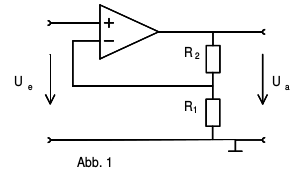
\includegraphics[width=0.5\textwidth]{schalt-1-1}
\end{center}
\begin{itemize}
% --- a) ---
\item[a)] F\"ur die Frequenz $f=1kHz$ und einen Verst\"arkungsfaktors $v=10$ bestimmen wir die maximale Eingangsspannung $u_e$, um eine unverzerrte Ausgangsspannung $u_a$ zu erhalten. \\
Wir haben eine maximale Eingangsspanung von $u_e=2.7V$ ermitteln k\"onnen.
\newpage
% --- b) ---
\item[b)] Die dargestellte Kennlinie stellt die Frequenz $u_a=f(u_e)$ dar. \\
\begin{center}
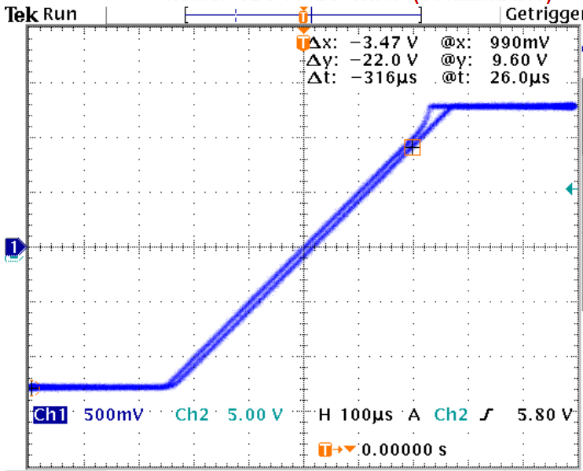
\includegraphics[width=0.7\textwidth]{3}
\end{center}
% --- c) ---
\item[c)] Der Amplitudengang $u_a(f)$ im einfach-logarithmischen Ma\ss{}stab \\
\begin{center}
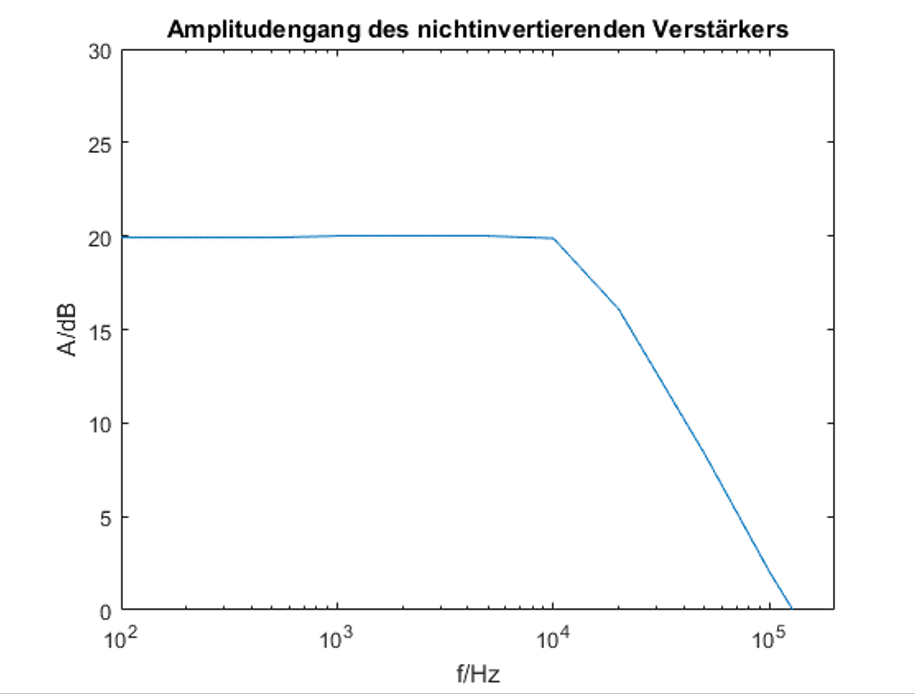
\includegraphics[width=0.9\textwidth]{4}
\end{center}
\end{itemize}
\newpage

% --- 1.2 ---
\subsection{Untersuchungen des Verhalten eines Impedanzwandlers}
In diesem Versuch skizzieren wir wieder den Amplitudengang im einfach logarithmischen Ma\ss{}stab mit folgender Schaltung:
\begin{center}
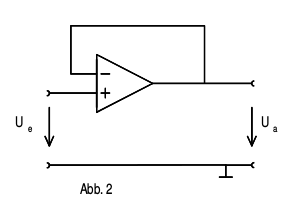
\includegraphics[width=0.5\textwidth]{schalt-1-2}
\end{center}
Der Amplitudengang sieht wie folgt aus:
\begin{center}
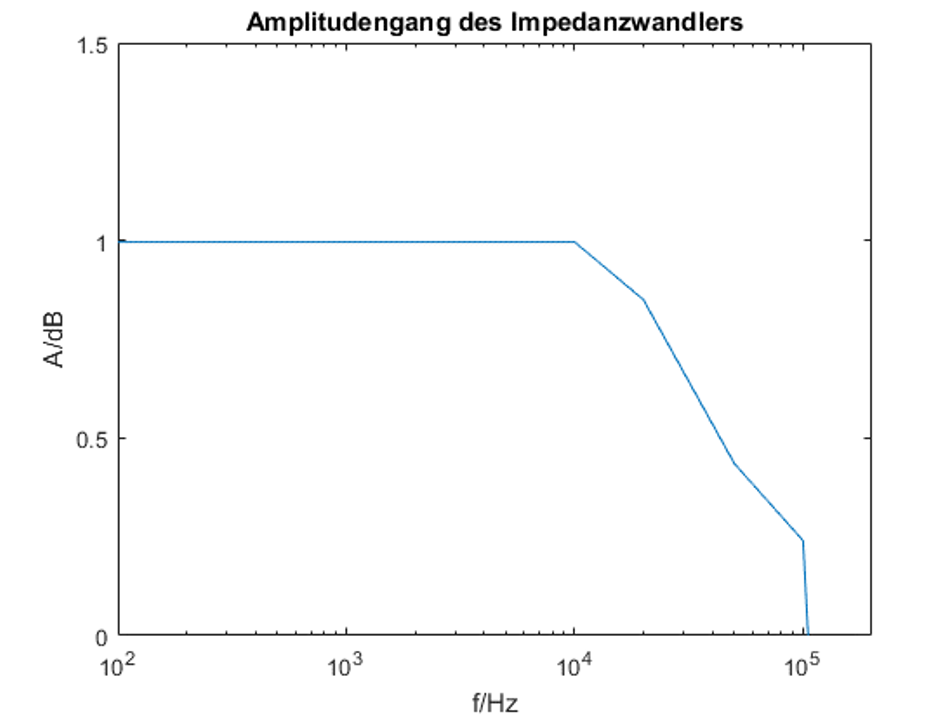
\includegraphics[width=0.7\textwidth]{6}
\end{center}
\newpage

% --- Aufgabe 2 ---
\section{Invertierender Verst\"arker}

\begin{itemize}
% --- a) ---
\item[a)] F\"ur die Frequenz $f=1kHz$ und einen Verst\"arkungsfaktors $v=10$ bestimmen wir die maximale Eingangsspannung $u_e$, um eine unverzerrte Ausgangsspannung $u_a$ zu erhalten. \\
Wir haben eine maximale Eingangsspanung von $u_e=2.6V$ ermitteln k\"onnen.
% --- b) ---
\item[b)] Die dargestellte Kennlinie stellt die Frequenz $u_a=f(u_e)$ dar. \\
\begin{center}
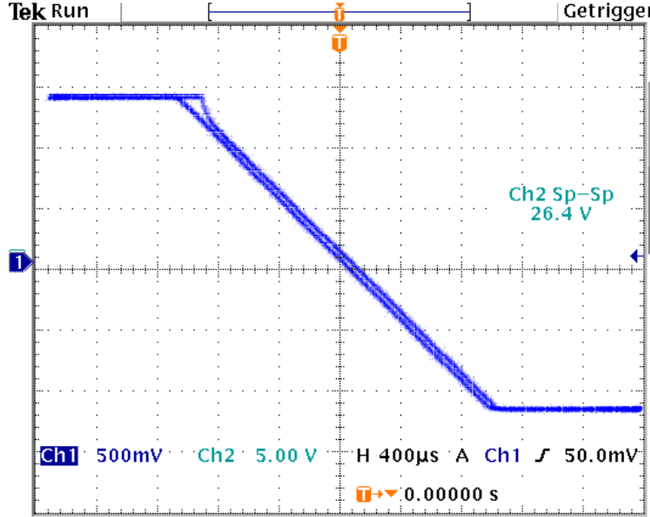
\includegraphics[width=0.7\textwidth]{8}
\end{center}
% --- c) ---
\item[c)] Der Amplitudengang $u_a(f)$ im einfach-logarithmischen Ma\ss{}stab \\
\begin{center}
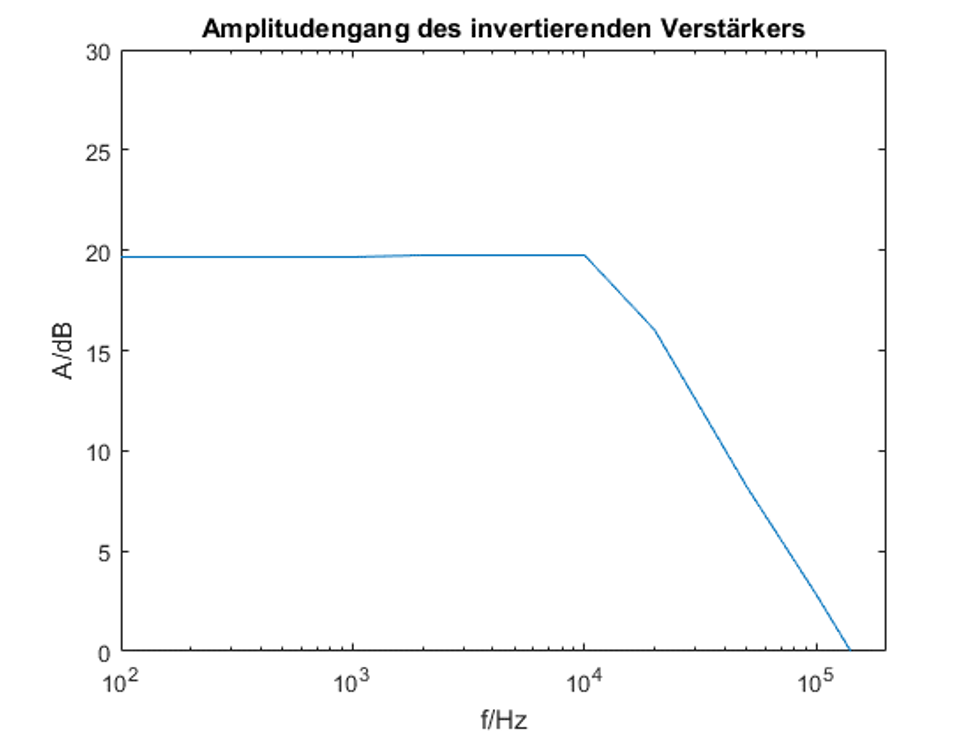
\includegraphics[width=0.7\textwidth]{9}
\end{center}
\end{itemize}

\newpage

% --- Aufgabe 3 ---
\section{Nicht-invertierender Schmitt-Trigger}
Nun werden die Eing\"ange des OP vertauscht. \\[1ex]
Die Schaltung verh\"alt sich jetzt wie ein Schmitt-Trigger und es gilt: \\
$U_{e,ein}=-(\frac{R_1}{R_2}) \cdot U_{a,min}$ \\
$U_{e,aus}=-(\frac{R_1}{R_2}) \cdot U_{a,max}$ \\[1ex]
\begin{center}
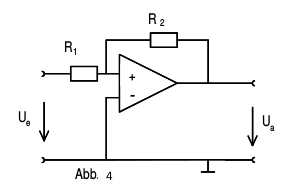
\includegraphics[width=0.5\textwidth]{schalt-3}
\end{center}
Wir stellen nun f\"ur die Frequenz $f=1kHz (Sinus)$ die Ein- und Ausgangsspannung dar.
\begin{center}
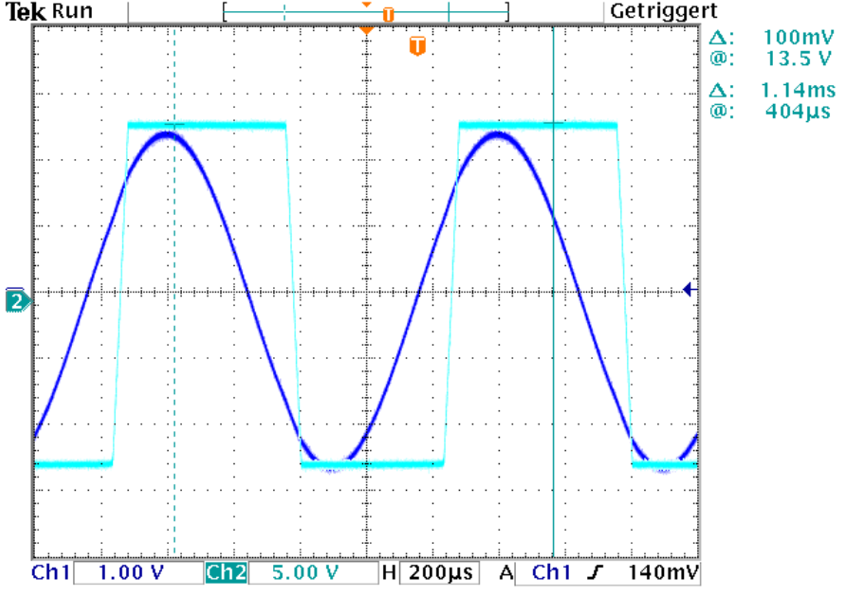
\includegraphics[width=0.7\textwidth]{10}
\end{center}

\newpage

\textit{Wie gro\ss{} ist bei dieser Beschaltung die Hysterese?} \\[2ex]
Im folgender Abbildung sehen wir die Hysterese:
\begin{center}
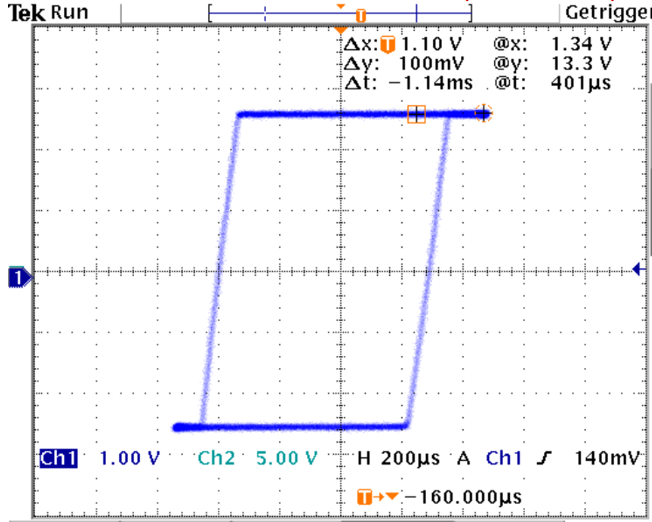
\includegraphics[width=0.7\textwidth]{11}
\end{center}
Die Eingangsspannung betr\"agt $U_{e,ein}=1.18V$ und die Ausgangsspannung $U_{e,aus}=-1.56V$. Aus dieser Differenz l\"asst sich die Hysterese errechnen. Sie betr\"agt $2.74V$.

\newpage

% --- Aufgabe 4 ---
\section{Integrator}
Die vorgegebene Eingangsschaltung integrieren wir mit folgender Schaltung.
\begin{center}
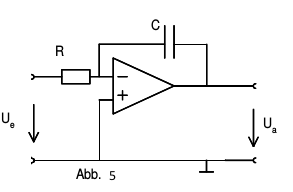
\includegraphics[width=0.5\textwidth]{schalt-4}
\end{center}
\begin{itemize}
\item[] Eingangssignal: Rechteck, $U_{pp}=2V$, $f=2kHz$
\item[] Bauteile: $R=10k\Omega$ und $C=0.1µF$
\end{itemize}
\textit{Bei der Integration einer Wechselspannung st\"ort der eventuell vorhandene Gleichanteil. Wie ist das Problem beherrschbar?} \\[1ex]
Die m\"ogliche St\"orung durch einen vorhandenen Gleichanteils k\"onnen wir umgehen, indem wir zum Aufbau eines Hochpasses einen Widerstand parallel zum Kondensator schalten.

\end{document}
